%TEMPLATE FILE
\documentclass{article}
\usepackage{graphicx} 
\usepackage{mathtools}
\usepackage{subcaption}
%usepackage[utf8]{inputenc}
\usepackage{siunitx}
\usepackage{pdfpages}
\usepackage{pdflscape}
\usepackage{float}
\usepackage{amsmath}
\usepackage{rotating}
\usepackage{geometry}
\usepackage{multicol}
\usepackage{xcolor}
\usepackage{pgfplots}
\usepackage[T1]{fontenc}
\usepackage[utf8]{inputenc}
\usepackage[icelandic]{babel}

\input{arduinoLanguage.tex}

\fontfamily{lmr}\selectfont

\graphicspath{ {images/} }

\usepackage{cite}



\usepackage{hyperref}
\usepackage{titlesec}
\usepackage{listings}
\definecolor{backcolour}{rgb}{0.95,0.95,0.92}
\definecolor{mygreen}{RGB}{28,172,0} % color values Red, Green, Blue
\definecolor{mylilas}{RGB}{170,55,241}

\lstset{language=C++,
    		backgroundcolor=\color{backcolour}, 
                basicstyle=\ttfamily,
                keywordstyle=\color{blue}\ttfamily,
                stringstyle=\color{red}\ttfamily,
                commentstyle=\color{orange}\ttfamily,
                morecomment=[l][\color{magenta}]{\#}
}

\lstset{language=Matlab,%
    %basicstyle=\color{red},
    backgroundcolor=\color{backcolour}, 
    breaklines=true,%
    morekeywords={matlab2tikz},
    keywordstyle=\color{blue},%
    morekeywords=[2]{1}, keywordstyle=[2]{\color{black}},
    identifierstyle=\color{black},%
    stringstyle=\color{mylilas},
    commentstyle=\color{mygreen},%
    showstringspaces=false,%without this there will be a symbol in the places where there is a space
    numbers=left,%
    numberstyle={\tiny \color{black}},% size of the numbers
    numbersep=9pt, % this defines how far the numbers are from the text
    emph=[1]{for,end,break},emphstyle=[1]\color{red}, %some words to emphasise
    %emph=[2]{word1,word2}, emphstyle=[2]{style},    
}
\setcounter{secnumdepth}{4}

\hypersetup{
    colorlinks=true, % make the links colored
    linkcolor=blue, % color TOC links in blue
    urlcolor=red, % color URLs in red
    linktoc=all % 'all' will create links for everything in the TOC
    pdftitle={Sharelatex Example},
    bookmarks=true,
    pdfpagemode=FullScreen,
}
\hypersetup{
    colorlinks=true, % make the links colored
    linkcolor=blue, % color TOC links in blue
    urlcolor=red, % color URLs in red
    linktoc=all % 'all' will create links for everything in the TOC
    pdftitle={Sharelatex Example},
    bookmarks=true,
    pdfpagemode=FullScreen,
    linkcolor=red,
}


\lstset{frame=single, numbers=left, numberblanklines=false, tabsize=2, linewidth= 1.1\linewidth, breaklines= true}
\begin{document}
	\pagenumbering{gobble}
\begin{titlepage}

\newcommand{\HRule}{\rule{\linewidth}{0.5mm}} % Defines a new command for the horizontal lines, change thickness here

\center % Center everything on the page
 
%----------------------------------------------------------------------------------------
%	HEADING SECTIONS
%----------------------------------------------------------------------------------------

%


\textsc{\LARGE Tækniskólinn í Reykjavík}\\[0.5cm] % Name of your university/college
\textsc{\large Grunndeild rafiðna}\\[0.5cm] % Minor heading such as course title
\textsc{\large í samstarfi við}\\[0.5cm]
\textsc{\LARGE Hochschule Ravensburg-Weingarten}\\[0.5cm] % Major heading such as course name

%----------------------------------------------------------------------------------------
%	TITLE SECTION
%----------------------------------------------------------------------------------------

\HRule \\[0.4cm]
{ \huge \bfseries Piezo-based string instrument pickup using $\mu$controller platform}\\[0.4cm] % Title of your document
\HRule \\[0.4cm]
 %{  \bfseries Bachelor Thesis}\\[1.5cm] % Title of your document
%----------------------------------------------------------------------------------------
%	AUTHOR SECTION
%----------------------------------------------------------------------------------------

\begin{minipage}{0.4\textwidth}
\begin{flushleft} \large
\textbf{\emph{Author:}}\\
Þorri Líndal {Guðnason} \\ % Your name 
\textbf{\emph{Matrikel:}} \\
29404 \\
\textbf{\emph{Contact:}} \\
thorrigu19@tskoli.is
\end{flushleft}
\end{minipage}
~
\begin{minipage}{0.4\textwidth}
\begin{flushright} \large
\textbf{\emph{Supervisor I:}} \\
Prof. Dr. rer. nat. Markus \textsc{Pfeil}\\ % Supervisor's Name 
\textbf{\emph{Supervisor II:}} \\
Baldur \textsc{Thorgilsson} % Supervisor's Name
\end{flushright}
\end{minipage}\\[2cm]

% If you don't want a supervisor, uncomment the two lines below and remove the section above
%\Large \emph{Author:}\\
%John \textsc{Smith}\\[3cm] % Your name

%----------------------------------------------------------------------------------------
%	DATE SECTION
%----------------------------------------------------------------------------------------

{\large \today}\\[1cm] % Date, change the \today to a set date if you want to be precise

%----------------------------------------------------------------------------------------
%	LOGO SECTION
%----------------------------------------------------------------------------------------

\includegraphics[scale=1.5]{logos2.png}\\[1cm] % Include a department/university logo - this will require the graphicx package
 
%----------------------------------------------------------------------------------------

\vfill % Fill the rest of the page with whitespace

\end{titlepage}
	\newpage
\newgeometry{left=3cm,bottom=0.1cm}
	\pagenumbering{arabic}
	\tableofcontents
\restoregeometry
	\newpage
%texti osfrv hér



%----------------------------------------------------------------------------------------
%	Kafli 1
%----------------------------------------------------------------------------------------
\bibliography{bs-citations} 
\section{Inngangur}
\label{chapter}
\subsection{Hvað er Piezo?}
\begin{flushleft}
As the structure of the piezo is crystal with special properties that can generate a voltage from the pressure of crystallization. We can use it instead of the general microphone by By which it can respond to vibrations and high sensitivity. When considering the structure of the acoustic guitar. Guitar body is wood and is designed to be hollow. When players strum guitar strings which is designed to the size and tension of the lines are different. by patterns of the sound of music. In science, When an object vibrates at any frequency. Would become a sound wave. That sound wave will travel through the structure of the wood body guitar. When we put the piezo speaker set up on the structure of guitar body is made of piezo crystals have better string vibration of the guitar itself. The piezo will generate a small voltage to which we can put to use in the future.
\end{flushleft}

 \begin{figure}[H]
  	\centering
  	\includegraphics[width=1\linewidth]{gamma2.png}
  	\caption{description}
 	 \label{figure1}
\end{figure}

\newpage
\section{Kóði fyrir prufun á Piezo}

\begin{flushleft}Þetta er kóðinn sem ég notaði til að prufa piezo-skynjarann í gegnum hliðræna innganginn á Arduino tölvunni og gerði graf í serial monitor
\end{flushleft}

\begin{lstlisting}[language=Arduino,caption=Kóði fyrir serial plotter, frame=none,label=code-serial]
void setup() {
  Serial.begin(9600);
}

void loop() {
  Serial.println(analogRead(A0));
  delay(2);
}

  Serial myPort;     
  int xPos = 1;         
  float inByte = 0;

  void setup () {
    size(400, 300);
    println(Serial.list());
    myPort = new Serial(this, Serial.list()[0], 9600);
    myPort.bufferUntil('\n');
  }
  void draw () {
    stroke(127, 34, 255);
    line(xPos, height, xPos, height - inByte);
    if (xPos >= width) {
      xPos = 0;
      background(0);
    } else {
      xPos++;
    }
  }
  void serialEvent (Serial myPort) {
    // get the ASCII string:
    String inString = myPort.readStringUntil('\n');

    if (inString != null) {
      inString = trim(inString);
      inByte = float(inString);
      println(inByte);
      inByte = map(inByte, 0, 1023, 0, height);
    }
  }
\end{lstlisting}
\newpage

\subsection{Piezo inngangur}
\begin{flushleft}
Það þurfti einfaldlega að tengja \textbf{piezo} við Arduino tölvuna þar sem plúsinn var tengdur í \textbf{GND} á Arduino tölvunni en mínusinn í Analog innganginn.  Piezo úr þremur reykskynjurum frá þremur mismunandi framleiðundum virkuðu allir í sitthvoru lagi við að lesa hristing sem inngang við \textbf{\textit{Analog(0)}}. 
\end{flushleft}

\begin{figure}[H]
 \label{Piezo-inn}

\begin{center}
\tikz{
\begin{axis}
[
     width=16cm,  height=10cm,
    title=Piezo serial inngangur:,
    xlabel={$Time$},
    ylabel={$Vin$},
]
    \addplot [blue] table {graph.txt};
\end{axis}
}
\end{center}
\end{figure}

\newpage %%%%%%%%

\subsection{Piezo útgangur}

\begin{flushleft}
Ég ákvað líka að prufa að senda hljóð út um Piezo út um hliðræna útganginn á Arduino tölvunni,  rétt eins og seinast virkuðu allir þrír sitthvorir eins og búist var við.  Það er heppilegt að það er innbygður kóði fyrir einmitt þetta í Arduino IDE sem heitir einfaldlega \textbf{"ToneMelody.h"}.  Kóðinn er í heild sinni hér fyrir neðan,  mjög einfaldur og notast við library sem heitir einfaldlega 'pitches' og er listi af tónum kortlagt við tíðnir. 



\begin{lstlisting}[language=Arduino, caption=Tone Melody Kóði, frame=none,label=generatedcode] 
int melody[] = {
  NOTE_C4, NOTE_G3, NOTE_G3, NOTE_A3, NOTE_G3, 0, NOTE_B3, NOTE_C4
};

int noteDurations[] = {
  4, 8, 8, 4, 4, 4, 4, 4
};

void setup() {

  for (int thisNote = 0; thisNote < 8; thisNote++) {

    int noteDuration = 1000 / noteDurations[thisNote];
    tone(8, melody[thisNote], noteDuration);

    int pauseBetweenNotes = noteDuration * 1.30;
    delay(pauseBetweenNotes);
    noTone(8);
  }
}

void loop() {
}

\end{lstlisting}
\end{flushleft}
\newpage %%%%%%%%

\section{Formagnari (LT072)}

\subsection{Rásamynd af formagnaranum}
\begin{flushleft}
Hristingurinn frá gítarnum gæti hreyft piezo-skynjarann nógu mikið til þess að senda frá sér mjög dauft merki. Merkið kemur inn um 3.5mm jack tengi í gegnum C1 þéttirinn inn í pinna 3 á TL071 rásinni sem þjónar sem magnari fyrir merkið frá piezo-skynjaranum og gain er áætlað af hlutfallinu á milli viðnámi R5 og R3,  sem sjást á \ref{schematic-preamp}

 \begin{figure}[H]
  	\centering
  	\includegraphics[width=1\linewidth]{schema.png}
  	\caption{Rásateikning fyrir formagnarann}
 	 \label{schematic-preamp}
\end{figure}
\end{flushleft}

\newpage
\subsection{3D teikning af rásinni}
 \begin{figure}[H]
  	\centering
  	\includegraphics[scale=0.125]{Formagnari-3D.png}
  	\caption{3D Teikning af rásinni}
 	 \label{schematic-preamp-3D}
\end{figure}
\newpage

\section{Samsetning á bretti}
\begin{flushleft}
Rásin sjálf endaði minni en búist var við en það er bara betra, skar út part af vello bretti rúmlega 1.5x2cm á stærð (mynd \ref{vello-ras}), næst þurfti bara að lóða alla víra og innganga við brettið. Hún var á endanum nógu lítil til að passa í gamalt myntubox sem ég átti til og ég vissi að myndi hýsa 9V batterí án vandræða.  (mynd \ref{altoids-lokad})  \par



\end{flushleft}
 \begin{figure}[H]
  	\centering
  	\includegraphics[scale=0.5]{vello-ras.png}
  	\caption{Formagnara rásinn samsett}
 	 \label{vello-ras}
\end{figure}

 \begin{figure}[H]
  	\centering
  	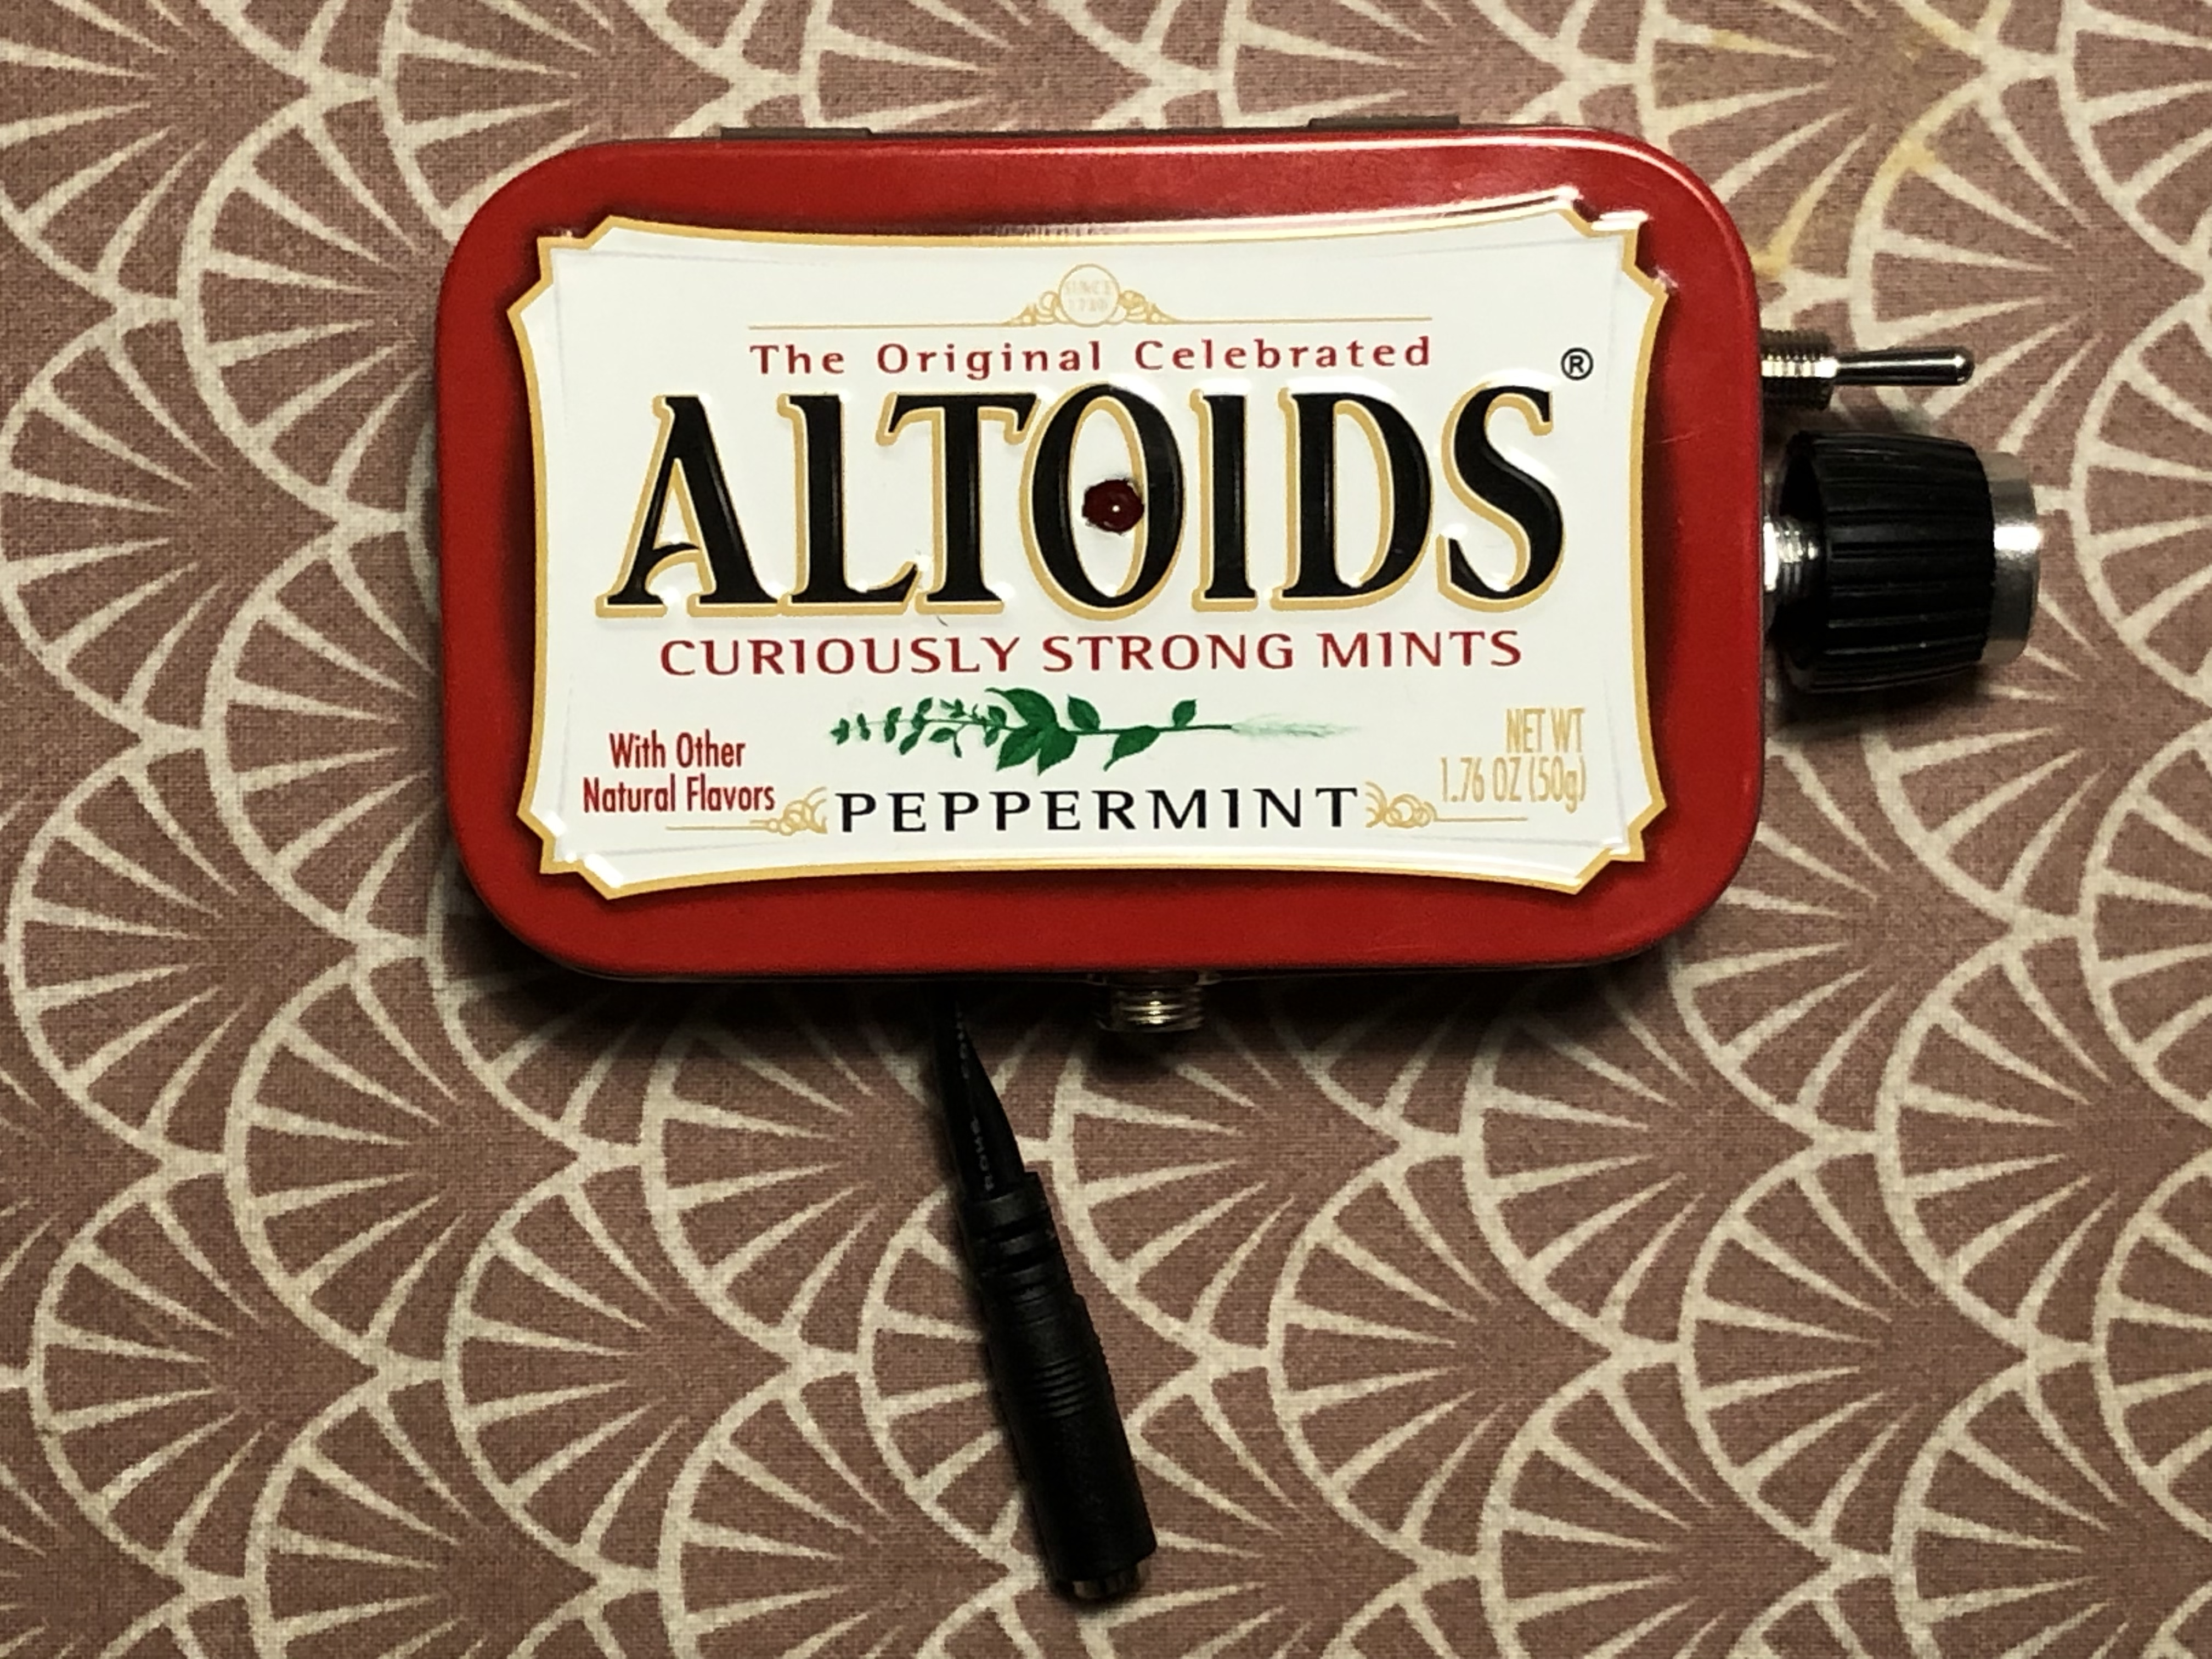
\includegraphics[scale=0.12]{altoids-lokad.png}
  	\caption{Formagnarinn kominn í myntu box}
 	 \label{altoids-lokad}
\end{figure}

 \begin{figure}[H]
  	\centering
  	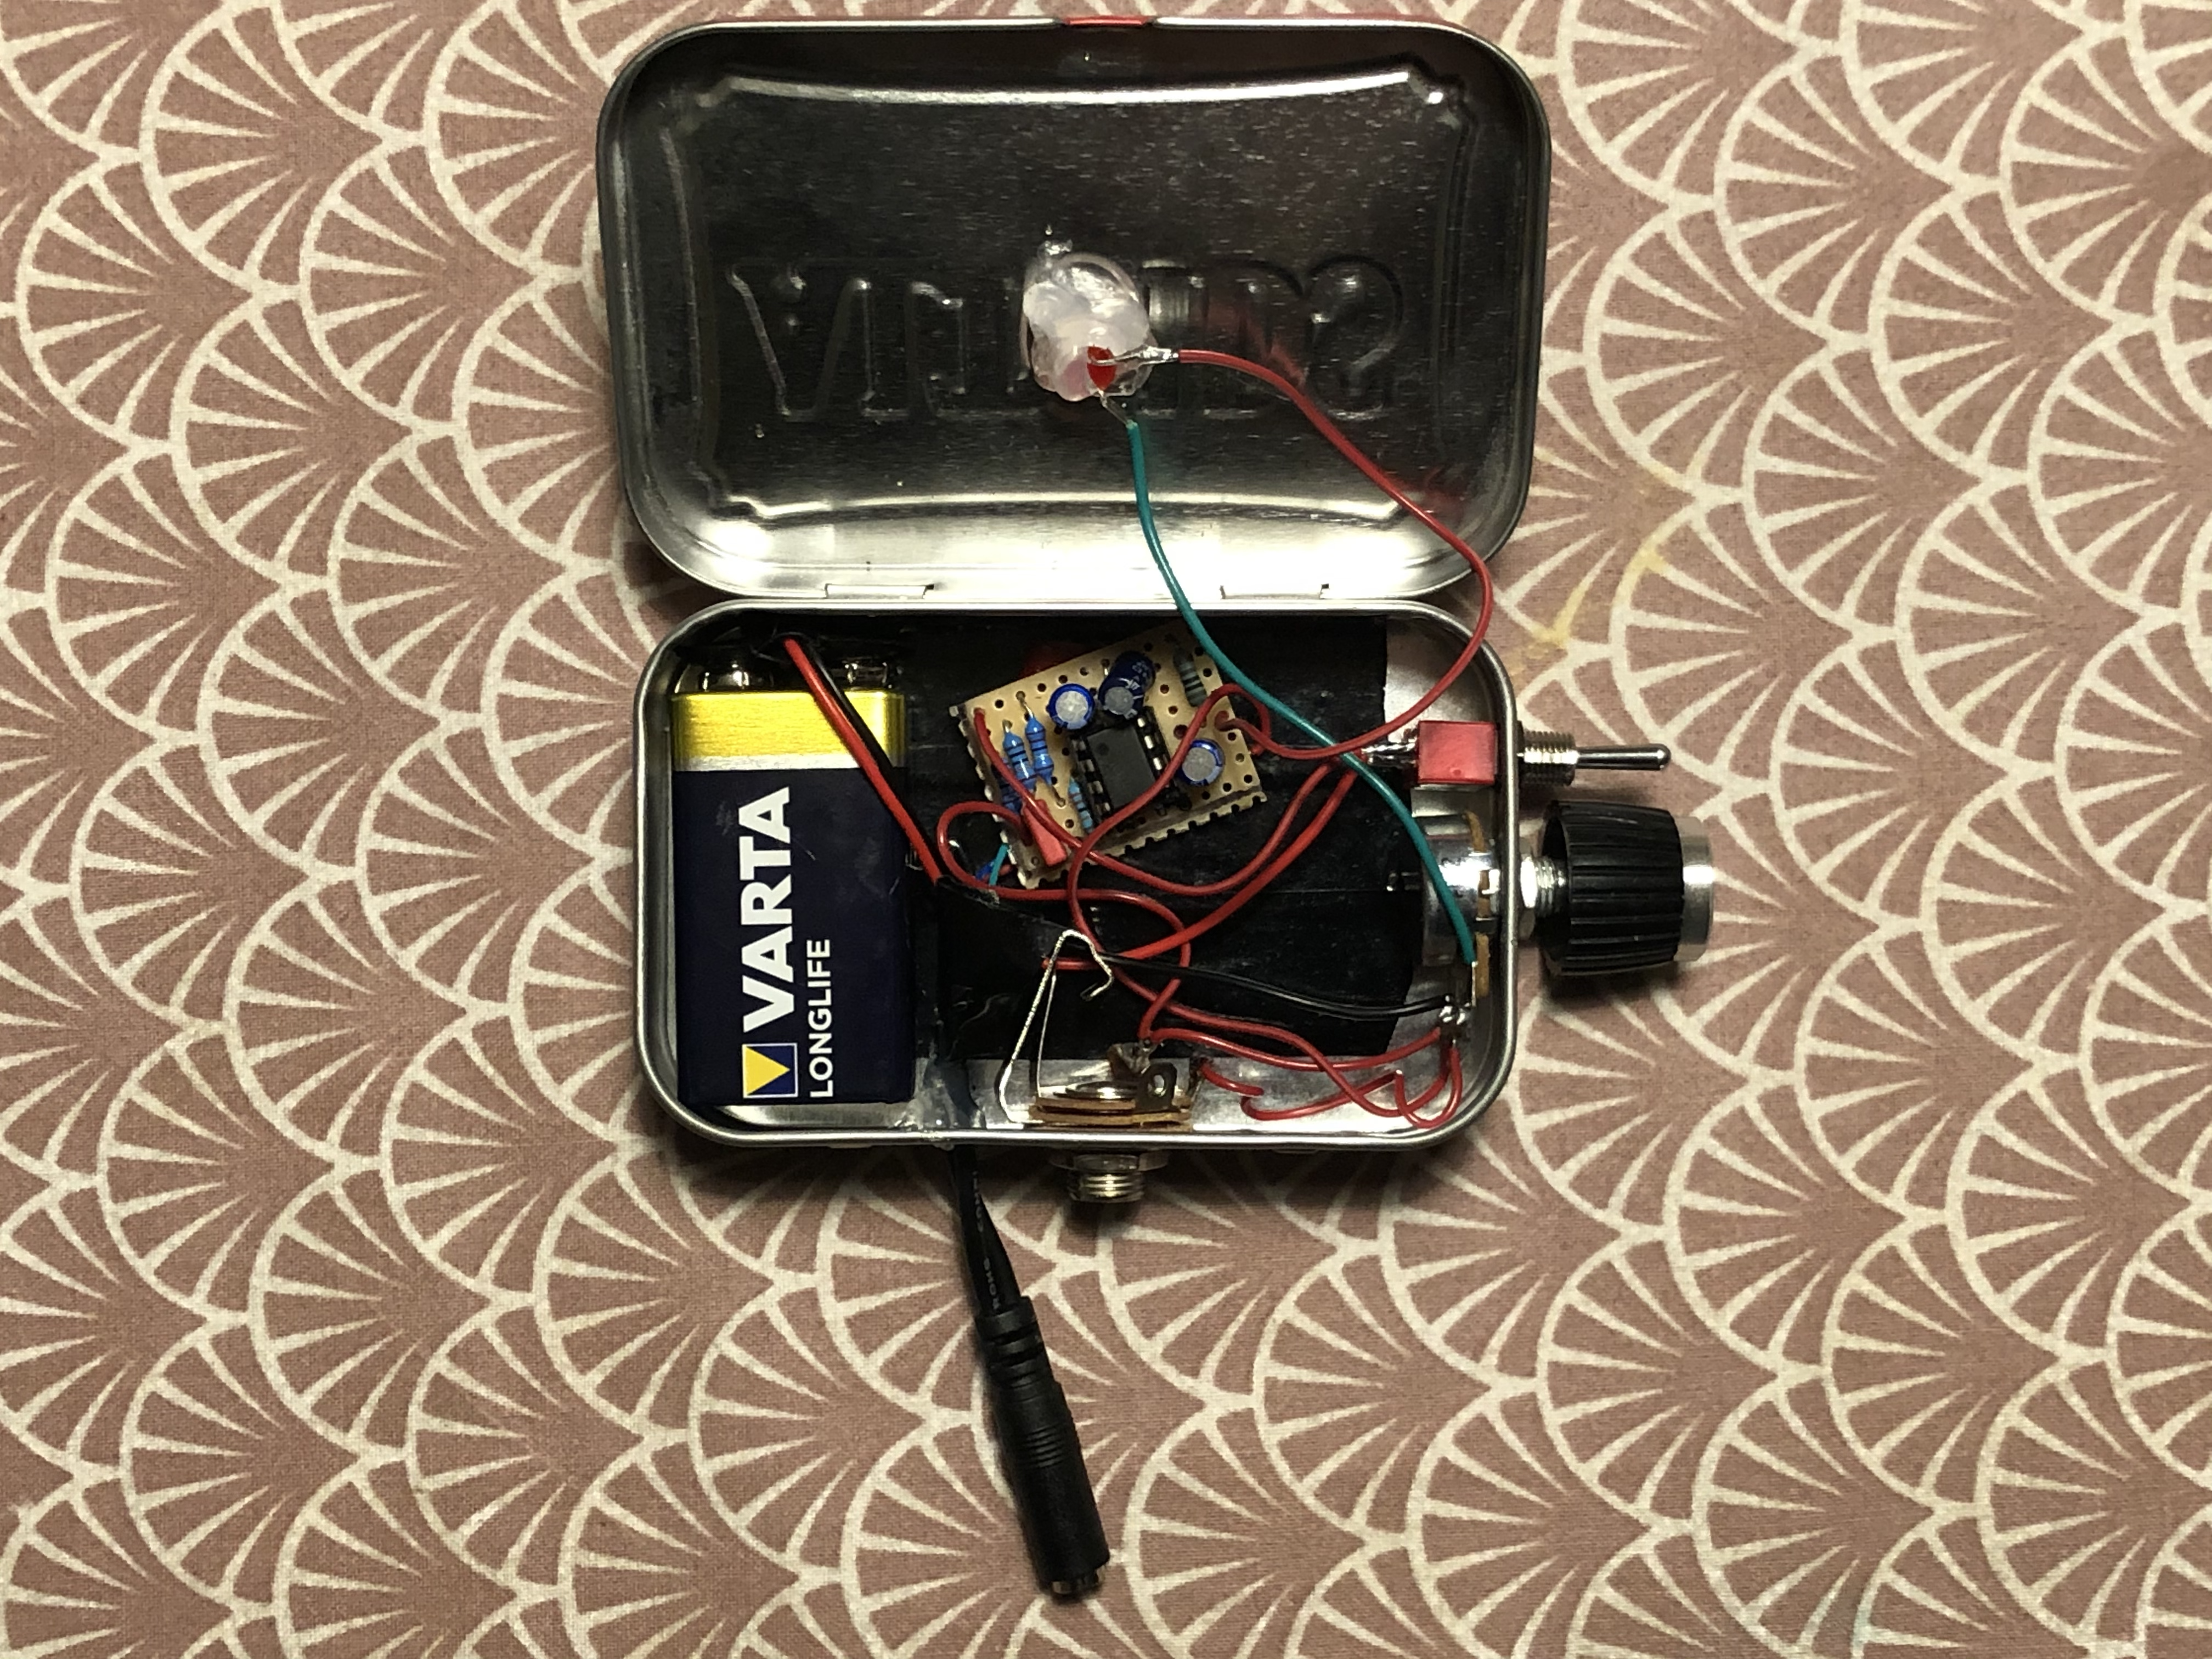
\includegraphics[scale=0.12]{Altoids-opid.png}
  	\caption{'Gut' mynd af formagnaranum}
 	 \label{altoids-opid}
\end{figure}

 \begin{figure}[H]
  	\centering
  	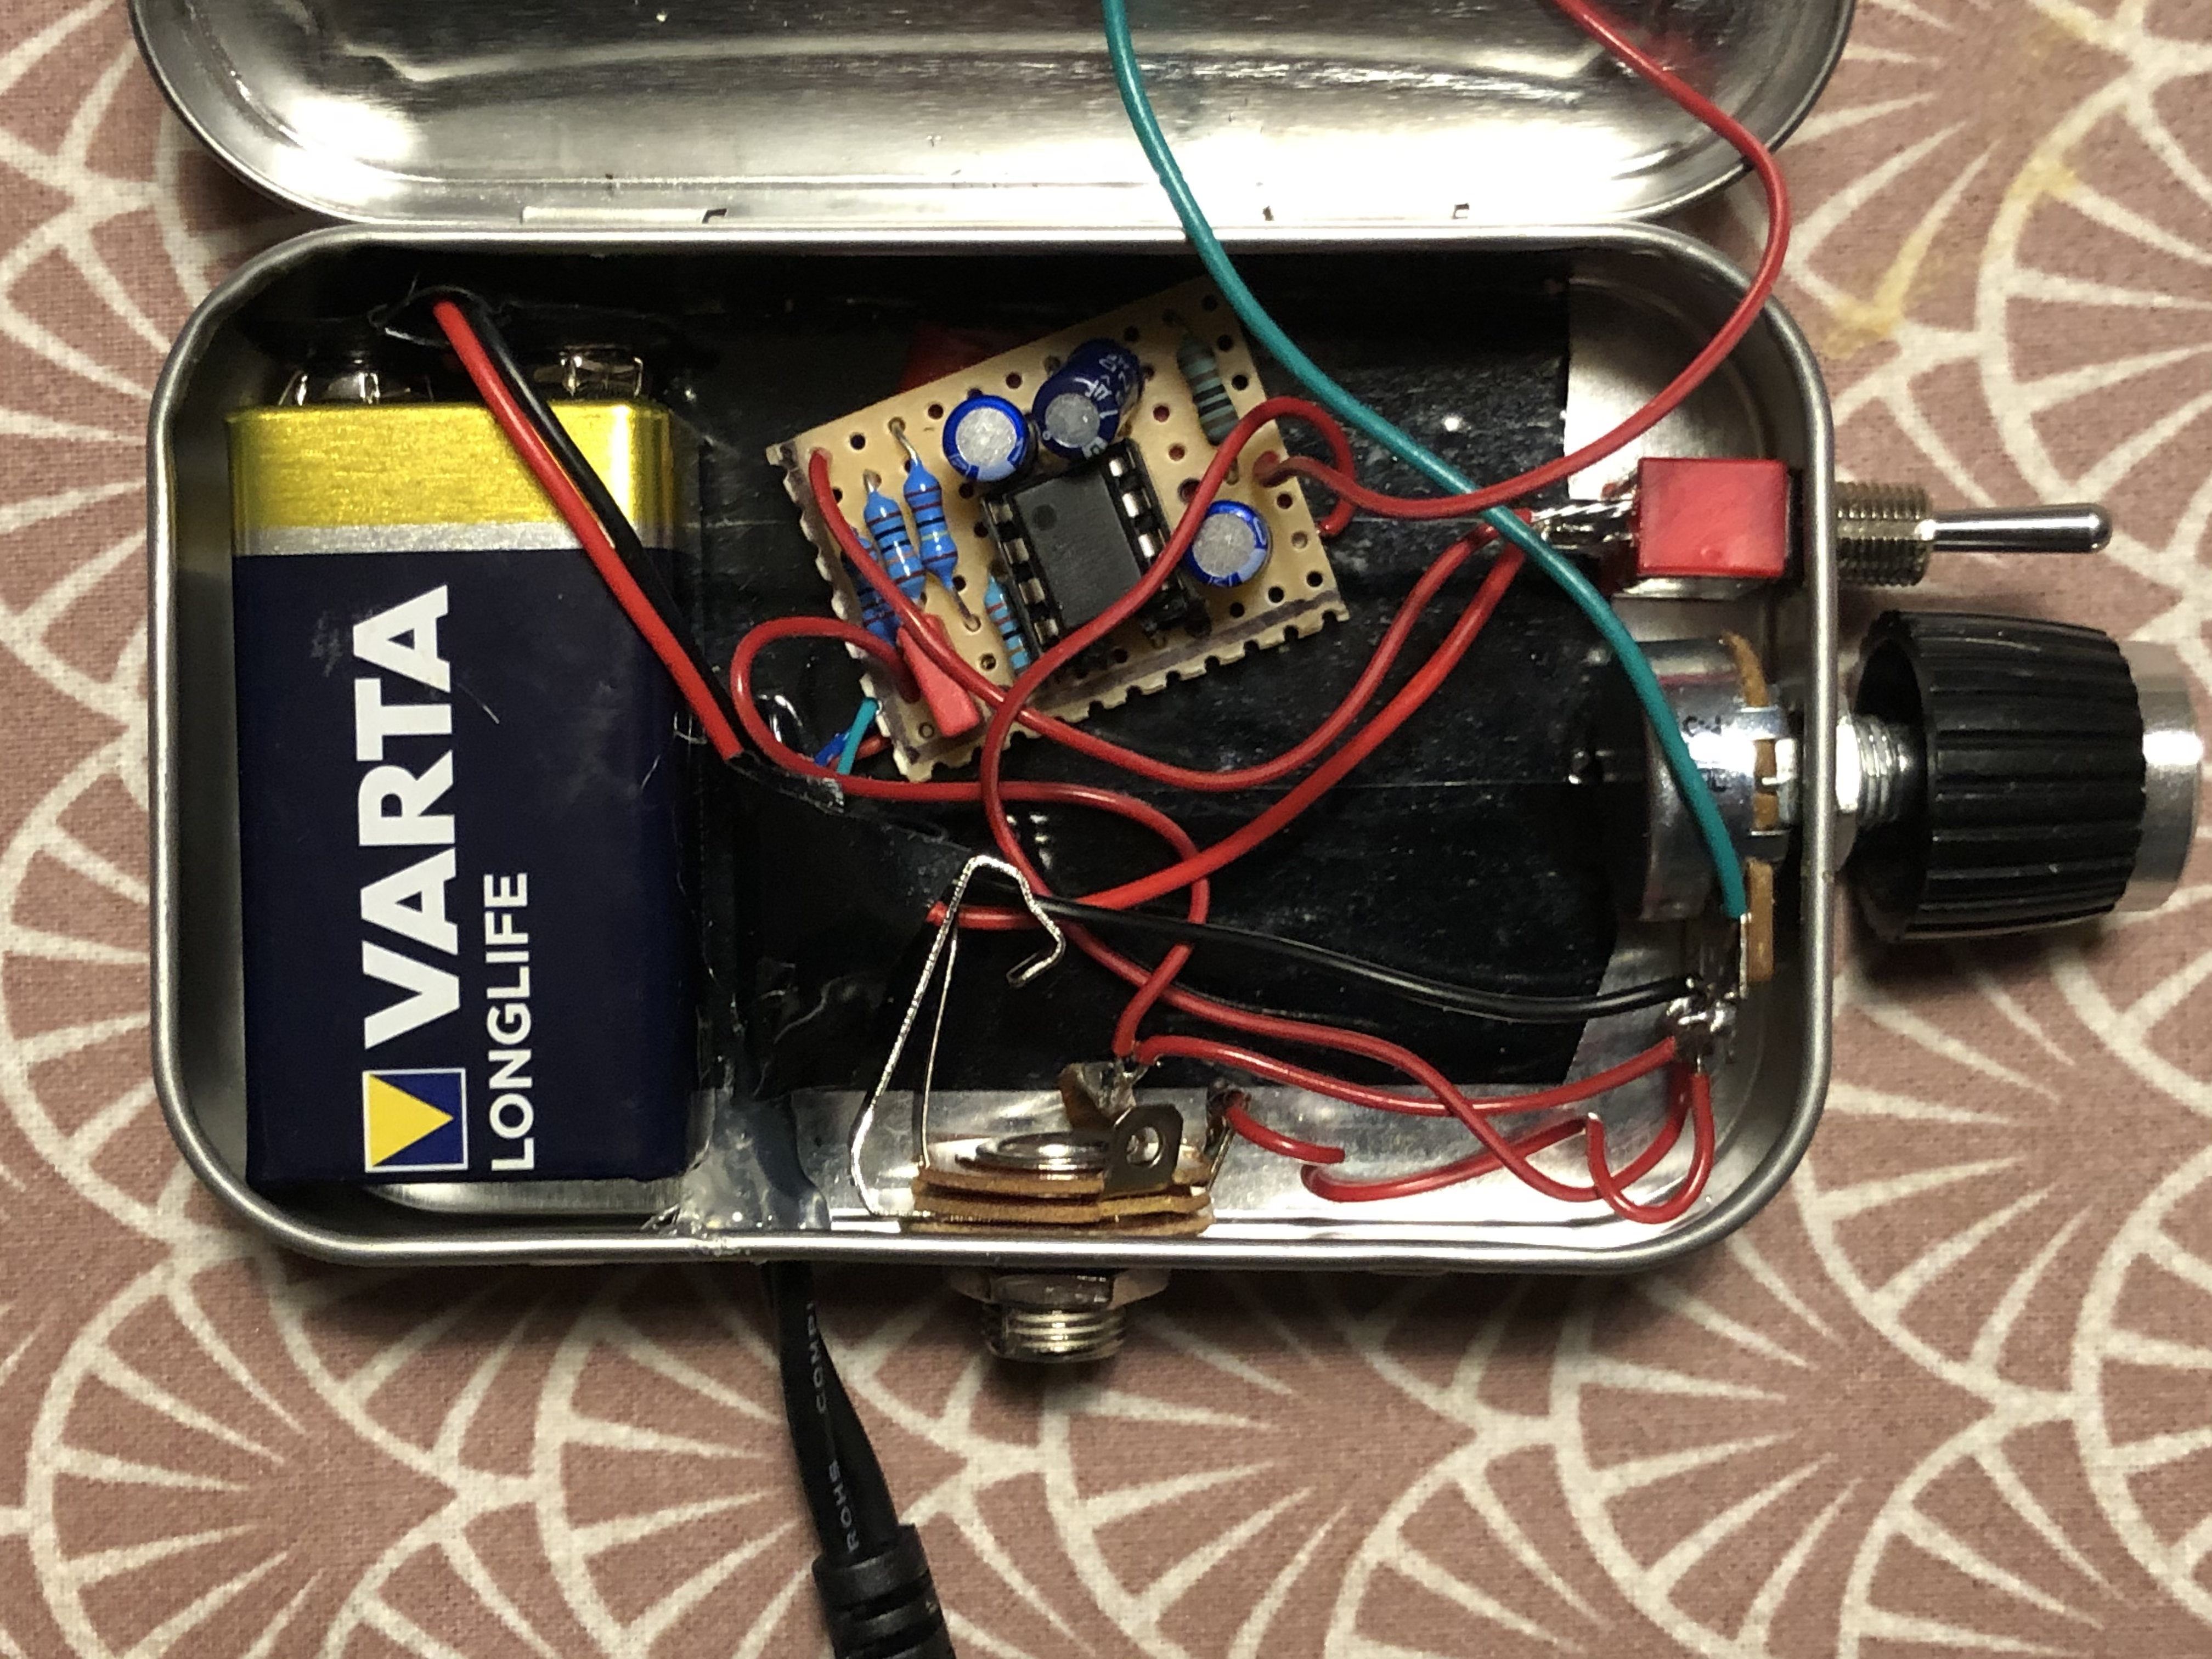
\includegraphics[scale=0.12]{Altoids-naer.png}
  	\caption{Nærmynd af formagnaranum}
 	 \label{altoids-naer}
\end{figure}

\newpage

\section{prufun á hljóðgæðum}

\begin{flushleft}
Upprunalega hugmyndin var að spila hvítt suð í gegnum hátalara á piezo-skynjarann og tengja hann inn í hliðræna innganginn á Arduino uno tölvunni og nota svo gögnin úr serial plotter til að reikna út tíðnisvörunina í Matlab en það virkaði ekki nógu vel svo ég ákvað frekar að nota tíðnisviðsmælinguna e. frequency analyzer) í sveiflusjá.
\end{flushleft}


\bibliographystyle{plain}

\end{document}